% =====================================================================
%  Dense Retrieval Is Degenerate Associative Memory
% =====================================================================
%  TARGET: TMLR (primary). Acceptance criteria are "claims supported by
%  evidence" + "interesting to some audience", with no novelty bar -- which is
%  exactly the shape of this paper. JMLR is the stretch; see
%  docs/05_VENUE_STRATEGY.md.
%
%  SUBMISSION IS DOUBLE-BLIND. The author block below stays anonymous until
%  camera-ready; the de-anonymised block is kept commented out directly beneath it.
%
%  EVERY NUMBER IN THIS PAPER TRACES TO docs/10_EXPERIMENT_LEDGER.md BY ID.
%  Before submission, regenerate every table from experiments/results/*.json with
%  scripts/make_tables.py rather than trusting the values typed here.
% =====================================================================

\documentclass[11pt]{article}
\usepackage[margin=1in]{geometry}
\usepackage{amsmath,amssymb,amsthm}
\usepackage{booktabs}
\usepackage{multirow}
\usepackage{tabularx}
\usepackage{graphicx}
\usepackage{xcolor}
\usepackage[numbers]{natbib}
\usepackage[colorlinks=true,allcolors=blue!55!black]{hyperref}

\newtheorem{proposition}{Proposition}
\newtheorem{lemma}{Lemma}
\newtheorem{corollary}{Corollary}
\theoremstyle{definition}
\newtheorem{claimbox}{Claim}
\theoremstyle{remark}
\newtheorem{remark}{Remark}

\newcommand{\ci}[2]{{\small[#1,\,#2]}}
\newcommand{\xid}[1]{\textsc{#1}}
\newcommand{\R}{\mathbb{R}}
\newcommand{\xib}{\boldsymbol{\xi}}
\newcommand{\lse}{\operatorname{lse}}
\newcommand{\sm}{\operatorname{softmax}}

\title{\bfseries Dense Retrieval Is Degenerate Associative Memory:\\
       A Reduction and a Regime Taxonomy for Agent Long-Term Memory}

\author{Anonymous Authors\\\small Paper under double-blind review}
% CAMERA-READY: replace the block above with the author list and affiliation.

\date{}

\begin{document}
\maketitle

\begin{abstract}
Agent long-term memory is almost universally retrieved by top-$k$ embedding similarity.
Associative-memory theory offers an alternative---recall as convergence to an attractor in
an energy landscape---but it has never been evaluated as the \emph{persistent memory
layer} of an agent under matched conditions. We first show why the two literatures have
not met: at the standard operating point they are the same operator. Proposition~1
establishes that dense top-$k$ retrieval is exactly the $(T{=}1,\ \beta\!\to\!\infty,\
b{=}0,\ R{=}I)$ corner of the modern Hopfield update, verified numerically on
$1000/1000$ queries on synthetic vectors and $838/838$ on real sentence embeddings. The industry baseline is
therefore a configuration of our own code rather than a separate system, which removes
implementation advantage by construction and converts an unanswerable question into a
sharp one: \emph{which departures from that corner pay for themselves, and where?}

We answer it across two modalities with a single frozen encoder, thread-disjoint
hyperparameter selection, and cluster-bootstrap intervals throughout: $5{,}847$ held-out
image queries, $1{,}977$ \textsc{LoCoMo} questions, $146$ multi-target text questions, and
$10{,}638$ temporal-association probes across two corpora. The answer is negative for
every mechanism that changes only \emph{how an answer is read off} a fixed landscape, and
the clearest evidence for that is the collapse of our own strongest positive result.
Iterative descent beat cosine by $+0.014$ pooled \ci{+0.006}{+0.021} on occluded images,
rising to $+0.021$ at 70\% occlusion. That number reproduces exactly and means much less
than we claimed: the metric is ten-way same-class accuracy, the cue's source image is
never in the bank, and at the selected $\beta$ the first descent step averages $12.7$
patterns out of $400$ with half the blend mass on the cue's own class --- an implicit
class vote. Scored against the matched baseline that makes explicit, a soft
$k$-nearest-neighbour class vote with no energy, no iteration and no attractor, descent is
\emph{worse} at every occlusion level ($-0.036$ pooled, \ci{-0.043}{-0.028}). Building the
experiment our premise actually describes --- occluded copies of images that \emph{are}
stored, scored by identity rather than class --- leaves descent at $-0.003$
\ci{-0.008}{+0.000} against cosine. Descent loses monotonically on conversational
question$\to$evidence retrieval as well: every increment costs accuracy, from $0.336$ to
$0.252$ Coverage@5 across an interpolation sweep whose endpoint provably reproduces cosine.

One premise explains every loss. Associative completion requires the cue to be a degraded
instance of a stored pattern, and question answering violates it. We nominated the
discriminating tests against ourselves and ran all three: masked spans of stored
\emph{text} satisfy the premise and give no $\beta$ that beats cosine in $45$ swept cells;
a cue that is a degraded copy of \emph{two} stored images at once loses $-0.245$; and
occluded copies of single stored images, the premise's best case, are the null above.
The premise therefore predicts every loss we measure and retains \emph{no} confirming
instance --- we report it as necessary and not sufficient, and withdraw the image result
as evidence for an associative mechanism.

We further show that $\beta$---the only dial with leverage---is influential only inside a
narrow, encoder-specific band (${\approx}[32,64]$ on the vision backbone we measure it on), above which
descent degenerates into cosine --- at $\beta{=}512$ it returns cosine's own
memory on $99.4\%$ of queries. A comparison run above that band compares cosine against itself, which we
argue is a live hazard for this literature rather than a detail of ours. Of eight
mechanisms tested beyond the reduction corner, exactly one survives: a nonparametric
predictor over the agent's own observed transitions beats cosine on one-hop temporal
association, reproduced in three independent implementations on two corpora. On
\textsc{LoCoMo}, against a pooled bank of $5{,}882$ turns and over $5{,}233$ probes in $272$
sessions, it raises Recall@1 from $0.064$ to $0.107$ ($+0.043$, $[+0.036,+0.050]$,
$p<10^{-4}$; $+67\%$ relative) and Recall@5 from $0.174$ to $0.251$. The same experiment
kills the multi-hop extension: at two hops the effect is $-0.002$ $[-0.008,+0.004]$,
$p{=}0.77$, and we withdraw a previously recorded $+0.185$ two-hop result of our own as an
artifact. Multi-step descent, residual peeling, repulsive parallel descent,
vote-count readout, multi-scale $\beta$, per-memory $\beta$, retrieval-margin calibration,
and coupling the predictor into the energy functional all fail, each with a diagnosed
mechanism rather than a bare null.

Finally, we report the measured magnitude of seven protocol errors we committed and
corrected. Each would have yielded a publishable but false result: a non-dimensionless
hyperparameter ($0.016$ vs.\ $0.277$ after normalisation), a pseudo-replicated bootstrap
($p{=}0.0005$ vs.\ $p{=}0.076$), test-set hyperparameter selection ($+0.042$ vs.\
$+0.004$), asymmetric candidate exclusion (an exact $0.000$ that read as a finding), an
unmatched step size ($-0.115$ vs.\ $-0.062$), and a significant result whose script was
never committed and does not reproduce ($+0.049$, $p{=}0.032$ vs.\ $+0.024$, $p{=}0.24$).
Two of the seven were false \emph{negatives}, which proved materially harder to find. We release all code, the regime taxonomy, and
an append-only experiment ledger in which every entry above appears with its date, its
question, and the entries it overturned.

\end{abstract}

\section{Introduction}
% Owner: Pushkal. Write AFTER method and results.
% Beats, in order:
%   1. Agent memory matters and is growing (MemGPT, A-MEM, MemoryBank, MemOS)
%   2. Retrieval is near-universally cosine top-k -- state this as the observation
%   3. Associative memory studies the retrieval OPERATOR, but on synthetic patterns
%   4. The two literatures have not met under controlled conditions. Say why: Prop 1
%      explains it -- at the standard operating point they are the SAME OPERATOR
%   5. Contributions C1-C4 as a bulleted list
%   6. A one-line honest preview of the headline finding, including what did NOT work


\section{Related Work}
% Owner: Rajit. ONLY cite entries marked VERIFIED in docs/07_CITATION_AUDIT.md.
%
% Three subsections:
%   3.1 Agent memory systems -- improve WHAT is stored, leave retrieval as similarity
%       MemoryBank, MemGPT, A-MEM, HippoRAG, MemOS, Titans, LightMem
%   3.2 Associative / energy-based memory -- study the OPERATOR
%       Hopfield 1982, Krotov & Hopfield 2016, Ramsauer 2020, Millidge 2022, DMHN
%   3.3 The 2026 convergence -- THE MOST IMPORTANT SUBSECTION, do not skip
%       PAM (Dury 2026)      -- association beyond similarity, but an EXTERNAL predictor
%       HeLa-Mem (ACL 2026)  -- Hebbian co-activation + episodic->semantic, but a GRAPH
%       DMHN                 -- context-modulated attractor geometry, but NO lifecycle
%       => each isolates one mechanism in a formalism that cannot express the other two.
%          That gap is our contribution. State it in exactly those terms.
%
% DO NOT write a related-work section that stops at Ramsauer 2020. Reviewers will know
% PAM and HeLa-Mem by name.


\section{The Reduction}
% Method. Owner: Pushkal.
%
% Section 3.1 is the most important half-page in the paper. It concedes the reviewer's
% strongest objection before they can raise it, and converts it into the paper's spine.
% See docs/06_RISK_REGISTER.md R-1.

\subsection{Memory as an energy landscape}

% Setup: memories m_i in R^d, L2-normalized, stacked as X in R^{d x N}.
% Query cue q; retrieval state xi initialized at q.
%
%   E(xi) = -lse(beta, X^T xi + b) + 0.5 ||xi||^2
%
% CCCP update (guaranteed descent):
%   xi <- X softmax(beta (X^T xi + b))
%   xi <- (1-eta) xi + eta R xi
%   xi <- xi / ||xi||
%
% TODO(Pushkal): state the three generalization axes G1/G2/G3 as a table here.

\subsection{Dense retrieval is a special case}

\begin{proposition}[Reduction]
\label{prop:reduction}
% For L2-normalized patterns, with T=1, b=0, R=I and beta -> infinity, the retrieval
% operator returns exactly argmax_i <q, m_i>, i.e. top-1 cosine retrieval.
%
% Proof: softmax(beta z) -> one-hot(argmax z) as beta -> inf; hence xi_1 -> m_{i*} with
% i* = argmax_i <q, m_i>. Readout by similarity to xi_1 returns m_{i*}.
\end{proposition}

% SAY THIS EXPLICITLY IN THE TEXT, do not leave it implicit:
%
%   "Proposition 1 means the standard dense-retrieval baseline is not an external
%    competitor but a point in our own parameter space. We therefore implement it as a
%    configuration of the same code path, which makes every comparison in Section 6 exact
%    by construction. The research question is not whether energy minimization beats
%    cosine similarity -- at that point they are the same operator -- but which
%    departures from it pay for themselves."
%
% Verified numerically: 1000/1000 queries agree with exact cosine top-1
% (tests/test_reduction.py, run in CI).

\subsection{Multi-target retrieval by residual peeling}

% docs/09_DAY0_FINDINGS.md F4/F5. This subsection reports a negative result and its fix.
%
% Descent converges to a single point xi*. Reading top-k by similarity to xi* ranks by
% proximity to ONE attractor, whereas the original query retains evidence for all k
% targets. Convergence therefore DESTROYS the multiplicity that top-k preserves --
% measured Recall 0.257 vs 1.000 at k=4 on synthetic data.
%
% Fix (Algorithm 1): descend, commit to the nearest attractor, project it out of the
% residual cue, re-descend. Matching pursuit over the energy landscape. Restores 1.000.
%
% This is a genuine contribution: no system in the related work performs multi-target
% readout under attractor dynamics. Present it as such, but present the failure first.

\subsection{Memory strength as basin depth}

% G2. b_i = w_u log(1+usage_i) + w_r exp(-dt_i/tau) + w_s surprise_i.
% Reinforcement, decay and forgetting become one term rather than three heuristics.
% MUST be compared against a cosine retriever given the SAME signals as a score prior --
% if that matches, this is engineering, not contribution. Say which it turned out to be.

\subsection{Learned associative topology}

% G3. R learned from temporal co-occurrence, NEVER from cosine similarity.
% Position carefully against PAM (Dury 2026), which already does association-beyond-
% similarity with an EXTERNAL predictor. Our claim is the INTEGRATION -- association
% reshapes the same landscape retrieval descends -- not the idea of association itself.
% See docs/07_CITATION_AUDIT.md.


\section{Experimental Protocol}
% Owner: Rajit. Mirror docs/04_EXPERIMENT_PROTOCOL.md exactly.
% Encoder (frozen, matched across ALL methods) | corpora | DegradeBench families
% Baselines + THE TUNING BUDGET GIVEN TO EACH (state this explicitly -- it pre-empts
% "you tuned yours and not theirs", the most common rejection reason for this shape).
% Seeds, CIs, hardware.


\section{Results}
\label{sec:results}

All numbers below are paired against the dense baseline of
Proposition~\ref{prop:reduction} on identical queries, with cluster-bootstrap intervals.
Ledger identifiers index \texttt{docs/10\_EXPERIMENT\_LEDGER.md}.

\subsection{Completion: descent beats cosine, and loses to a plain classifier}
\label{sec:completion}

\begin{table}[t]\centering\small
\caption{The image study with its matched baseline. The metric is \textbf{same-class top-1
accuracy} over ten classes, not identification, and the cue's source image is \emph{not} in
the bank --- see \S\ref{sec:occlusion}. $\beta$, $k$ and $\tau$ all selected on the same
disjoint tune half; one pre-committed paired test on the held-out half. $n{=}5{,}847$ query
instances from $1{,}949$ distinct images; bootstrap resamples images. $^{*}$CI excludes zero.}
\label{tab:images}
% GENERATED by scripts/make_tables.py -- do not edit
\begin{tabular}{@{}lrrrl@{}}
\toprule
\textbf{Occlusion} & \textbf{Cosine} & \textbf{Descent} ($\beta{=}40$) & \textbf{$k$-NN vote} ($k{=}20$) & \textbf{Descent $-$ vote (95\% CI)} \\
\midrule
30\% & 0.730 & 0.733 & 0.761 & $-0.028$ \ci{-0.040}{-0.017}$^{*}$ \\
50\% & 0.542 & 0.559 & 0.600 & $-0.041$ \ci{-0.054}{-0.027}$^{*}$ \\
70\% & 0.386 & 0.407 & 0.445 & $-0.038$ \ci{-0.052}{-0.024}$^{*}$ \\
\midrule
\textbf{pooled} & \textbf{0.553} & \textbf{0.566} & \textbf{0.602} & $\mathbf{-0.036}$ \ci{-0.043}{-0.028}$^{*}$ \\
\bottomrule
\end{tabular}

\end{table}

\begin{table}[t]\centering\small
\caption{Completion as the premise defines it (\xid{X113b}): cues are occluded copies of
images that \emph{are} in the bank, scored by \textbf{same-image} recall@1. Identity control
at $0\%$ occlusion: cosine recall@1 $=1.0000$. $\beta$ selected on a disjoint half of the
bank images and used once; selection chose $\beta{=}80$, the top of the grid. Same-class
accuracy on the identical cues is shown for comparison with Table~\ref{tab:images}.}
\label{tab:completion}
% GENERATED by scripts/make_tables.py -- do not edit
\begin{tabular}{@{}lrrlrrr@{}}
\toprule
& \multicolumn{3}{c}{\textbf{Same-image recall@1}} & \multicolumn{3}{c}{\textbf{Same-class accuracy}} \\
\cmidrule(lr){2-4}\cmidrule(lr){5-7}
\textbf{Occlusion} & Cosine & Descent & $\Delta$ (95\% CI) & Cosine & Descent & $\Delta$ \\
\midrule
30\% & 0.855 & 0.855 & $+0.000$ \ci{+0.000}{+0.000} & 0.915 & 0.915 & $+0.000$ \\
50\% & 0.635 & 0.630 & $-0.005$ \ci{-0.015}{+0.000} & 0.755 & 0.760 & $+0.005$ \\
70\% & 0.380 & 0.375 & $-0.005$ \ci{-0.015}{+0.000} & 0.545 & 0.535 & $-0.010$ \\
\midrule
\textbf{pooled} & \textbf{0.623} & \textbf{0.620} & $\mathbf{-0.003}$ \ci{-0.008}{+0.000} & 0.738 & 0.737 & $-0.002$ \\
\bottomrule
\end{tabular}

\end{table}

Table~\ref{tab:images} was for most of this project the paper's one clean positive for the
energy mechanism itself, and the first three columns are unchanged from that version:
descent beats cosine by $+0.014$ pooled, growing with corruption severity, on a
pre-committed held-out split. The fourth column is why we no longer report it that way. A
soft $k$-NN class vote --- selected on the same tune half, from a grid declared in advance
--- scores $0.602$ where descent scores $0.566$, and beats descent at every occlusion
level. \S\ref{sec:occlusion} gives the mechanism: on a \emph{class} metric, descent at
$\beta{=}40$ is an implicit class vote over $\approx 13$ neighbours, and an explicit vote
over $k{=}20$ does the same job better. Table~\ref{tab:completion} then asks the question
the metric name implied all along --- can descent retrieve the \emph{particular} stored
image a cue was degraded from --- and the answer is $-0.003$ \ci{-0.008}{+0.000}.

The latency comparison is unchanged and now lands differently: descent costs $21\times$
cosine's wall-clock latency ($0.0502$\,ms vs.\ $0.0024$\,ms per query) to be beaten by a
classifier that costs one extra argpartition.

Two further qualifications, which predate \xid{X113} and survive it. First, the apparent
advantage is \emph{capacity-dependent}: growing the bank from $100$ to $4{,}000$ patterns at
fixed $\beta{=}32$, cosine overtakes descent past $N\approx 800$. Second, descent's rank-1
gain over cosine comes with a \emph{shortlist regression}: recall@5 is $0.605$ against cosine's $0.759$
and MRR $0.589$ against $0.643$, all class-level (Table~\ref{tab:multibeta}). Converging to a single
attractor means ranks 2--5 measure proximity to that attractor rather than to the query,
which is Remark~\ref{rem:shortlist} and is now confirmed in three independent settings.

\paragraph{Two earlier verdicts of ours, withdrawn.} A previous version of this study used
$80$ distinct images with unpaired intervals roughly $5\times$ the effect size and $\beta$
tuned on the test images; those conclusions were underpowered and Table~\ref{tab:images}
supersedes them. The version that replaced it --- the one with the honest split, which we
described as a clean positive for the energy mechanism --- is withdrawn in turn by its own
fourth column. The number stands; the interpretation does not.

\subsection{Semantic match: every increment of descent costs accuracy}
\label{sec:semantic}

\begin{table}[t]\centering\small
\caption{\textsc{LoCoMo}, $1{,}977$ questions over $5{,}882$ turns. \texttt{anchor}
interpolates between pure cosine ($1.0$) and pure descent ($0.0$); the baseline is a point in
our own parameter space, so the sweep measures exactly what descent adds. The reduction check
passes $196/196$ at $\texttt{anchor}{=}1.0$.}
\label{tab:locomo}
% GENERATED by scripts/make_tables.py -- do not edit
\begin{tabular}{@{}lrl@{}}
\toprule
\textbf{Condition} & \textbf{Coverage@5} & \textbf{95\% CI} \\
\midrule
\textbf{$\texttt{anchor}{=}1.00$ \textit{(is cosine)}} & \textbf{0.336} & \ci{0.316}{0.355} \\
$\texttt{anchor}{=}0.90$, $\mathrm{pp}_0{=}32$ & 0.331 & \ci{0.311}{0.351} \\
$\texttt{anchor}{=}0.75$, $\mathrm{pp}_0{=}4$ & 0.321 & \ci{0.301}{0.340} \\
$\texttt{anchor}{=}0.50$, $\mathrm{pp}_0{=}4$ & 0.304 & \ci{0.285}{0.324} \\
$\texttt{anchor}{=}0.25$, $\mathrm{pp}_0{=}4$ & 0.273 & \ci{0.255}{0.292} \\
$\texttt{anchor}{=}0.00$, $\mathrm{pp}_0{=}4$ & 0.252 & \ci{0.234}{0.271} \\
energy, fixed $\beta{=}32$ & 0.236 & \ci{0.218}{0.254} \\
\bottomrule
\end{tabular}

\end{table}

Table~\ref{tab:locomo} is monotone: the optimum sits at the boundary where the method
\emph{is} the baseline. The table shows the best $\mathrm{pp}_0$ at each anchor; the worst
cell of the full sweep is $\texttt{anchor}{=}0.00,\ \mathrm{pp}_0{=}32$ at $0.201$
\ci{0.184}{0.218}, which is the broad-start annealing failure of \S\ref{sec:band} compounding
with the absent query anchor. There is no interior operating point at which descent helps on
question$\to$evidence retrieval, which is the dominant query type in deployed agent memory.

\paragraph{A data bug that invalidated an earlier result.} \textsc{LoCoMo} dialogue
identifiers are unique only \emph{within} a conversation: $5{,}882$ turns carry $1{,}033$
distinct identifiers, and $132$ of conversation~0's $134$ gold identifiers recur in other
conversations. Our first capacity sweep pooled banks without namespacing, so distractors
satisfied gold identifiers and scored as hits. Its headline---``adaptive $\beta$ improves as
the bank grows''---was an artefact; with namespaced identifiers adaptive $\beta$ \emph{degrades}
($0.250 \to 0.231$), merely less steeply than fixed $\beta$ ($0.244 \to 0.216$). We report
this because the failure mode is specific to this widely used benchmark and will recur.

\subsection{Composition: the one mechanism that works}
\label{sec:composition}

\paragraph{The gate.} Before building a predictor we checked whether cosine already solves
``what happened next''. It does not: Recall@1 is $0.105$ with the gold episode at median rank
$24$ of $1{,}319$. The failures are instructive---they are lexical collisions across
unrelated storylines, where a cue about a cottage drive returns ``forty minutes each way''
from an apartment-hunting thread. Oracle-restricting candidates to the correct storyline
still reaches only $0.488$, so the difficulty is not merely retrieval breadth. Temporal
succession is genuinely not a similarity relation (\xid{X16}).

\paragraph{The parametric predictor fails completely.} A low-rank JEPA predictor fitted on
some storylines and evaluated on others reaches Recall@1 of $1.000$ on the storylines it was
fitted on and $0.000$ on unseen ones, against the cosine baseline's $0.131$---worse
than doing nothing. No capacity escapes it: across ranks $2$ to $32$ the best unseen
Recall@1 at any setting is $0.016$, and the two largest capacities score exactly zero.
The diagnostic explains why: displacement vectors between consecutive episodes are
near-orthogonal (mean pairwise cosine $+0.004$) and the top ten principal
components carry only $31\%$ of their variance. There is no global ``and then''
direction to fit, and $134$ transitions in $768$ dimensions cannot teach one
(\xid{X17}, re-run as \xid{X17-r}). We report this as a result about inductive bias, not as
a tuning failure.

\paragraph{The nonparametric predictor works, on our corpus and on a public one.}
Equation~\eqref{eq:knnwm}, with $(k,\tau)$ selected on held-out storylines or sessions only,
beats cosine on one-hop association in three independent implementations
(Table~\ref{tab:assoc}). The third is the one that matters: it runs the same probe design on
\textsc{LoCoMo}, a benchmark built by another group, against the \emph{full pooled bank} of
$5{,}882$ turns from all ten conversations, so a prediction must beat distractors from nine
unrelated conversations as well as its own. Dialogue identifiers are namespaced by
conversation---without that, $5{,}882$ turns carry only $1{,}033$ distinct identifiers and
distractors satisfy gold identifiers, the bug described in \S\ref{sec:semantic}.

\begin{table}[t]\centering\small
\caption{One-hop temporal association. Three implementations, two corpora. ``Clusters'' is
the bootstrap resampling unit---storylines for the episodic corpus, sessions for
\textsc{LoCoMo}. Implementations (ii) and (iii) were written without reference to (i).
Absolute scores are lower on \textsc{LoCoMo} because the task is harder: a larger pooled
bank, nine conversations of distractors, and speaker-alternating turns. The relative effect
is \emph{larger} there.}
\label{tab:assoc}
% GENERATED by scripts/make_tables.py -- do not edit
\footnotesize\setlength{\tabcolsep}{4pt}
\begin{tabular}{@{}llrrccl@{}}
\toprule
& \textbf{Corpus} & \textbf{Probes} & \textbf{Clust.} & \textbf{Cosine} & \textbf{WM} & \textbf{Paired $\Delta$ R@1} \\
\midrule
(i) & episodic (ours), 50/50 & 123 & 61 & 0.106 & 0.130 & $+0.024$ \ci{-0.032}{+0.083}, $p{=}0.24$ \\
(ii) & episodic (ours), 4-fold & 257 & 122 & 0.105 & 0.140 & $+0.035$ \ci{+0.012}{+0.061}, $p{=}0.002$ \\
(iii) & \textbf{\textsc{LoCoMo}}, 4-fold & \textbf{5,233} & \textbf{272} & \textbf{0.064} & \textbf{0.107} & $\mathbf{+0.043}$ \ci{+0.036}{+0.050}, $\mathbf{p<10^{-4}}$ \\
\bottomrule
\end{tabular}

\end{table}

\begin{figure}[t]\centering
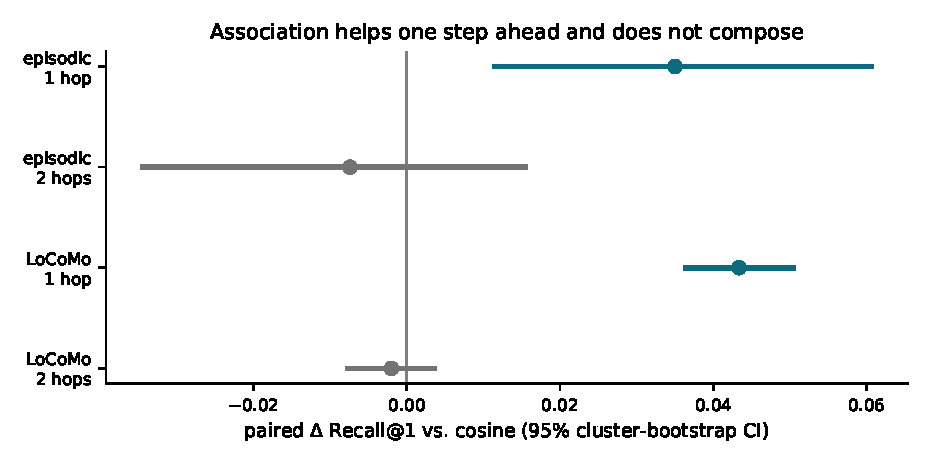
\includegraphics[width=0.78\textwidth]{figures/assoc_hops.pdf}
\caption{Paired $\Delta$ Recall@1 against cosine, both corpora, one and two hops. Intervals
are 95\% cluster bootstrap (storylines for the episodic corpus, sessions for
\textsc{LoCoMo}). The one-hop effect is positive on both corpora and larger on the public,
harder one; the two-hop effect is null on both. Generated by
\texttt{scripts/make\_tables.py}.}
\label{fig:hops}
\end{figure}

On \textsc{LoCoMo} the effect is $+67\%$ relative at Recall@1 and $+0.077$
\ci{+0.067}{+0.087} at Recall@5 ($0.174 \to 0.251$). This is the only claim in the paper with
external validity, and the only one reproduced three times; we weight it accordingly, and we
have restricted the paper's positive claims to it.

\paragraph{Multi-hop composition does not hold. We withdraw our own earlier result.}
An earlier run of ours indicated that iterating the predictor recovers two-hop chains it was
never trained on: Recall@5 of $0.446$ against cosine's $0.262$, $\Delta = +0.185$
\ci{+0.076}{+0.297}, $p<0.001$. That was the strongest result we had recorded. It does not
survive.

Three subsequent measurements (Table~\ref{tab:twohop}) return nulls, the last of them on
public data at $n{=}5{,}013$ with $272$ clusters---roughly $37\times$ the probe count of the
original. We therefore withdraw the two-hop claim as an artifact rather than suspending it.
The $+0.185$ figure should not be cited, including from our own ledger, where it now carries
a pointer to this result.

\begin{table}[t]\centering\small
\caption{Two-hop composition, every measurement we have. The original script was lost before
it was committed, so (a) cannot be re-run; (b) and (c) are independent reimplementations
under storyline- and session-disjoint rotation. Row (c) is $p{=}0.77$; the claim is withdrawn.}
\label{tab:twohop}
% GENERATED by scripts/make_tables.py -- do not edit
\footnotesize\setlength{\tabcolsep}{4pt}
\begin{tabularx}{\textwidth}{@{}l>{\raggedright\arraybackslash}X rc>{\raggedright\arraybackslash}X@{}}
\toprule
& \textbf{Corpus / protocol} & \textbf{Probes} & \textbf{Metric} & \textbf{Result} \\
\midrule
(a) & episodic, 50/50 \textit{(lost)} & 65 & R@5 & $0.446$ vs.\ $0.262$; $\Delta{+}0.185$ \\
(b) & episodic, 4-fold & 135 & R@5 & $0.230$ vs. $0.207$; spans zero \\
(c) & \textsc{LoCoMo}, 4-fold & 5,013 & R@1 & $0.041$ vs. $0.043$; $\Delta-0.002$ \ci{-0.008}{+0.004} \\
\bottomrule
\end{tabularx}

\end{table}

A residual signal does exist at two hops on \textsc{LoCoMo} at Recall@5 ($+0.012$
\ci{+0.004}{+0.019}), an order of magnitude below the one-hop effect and not visible at
Recall@1. We report it for completeness and do not build on it. The honest summary is that
association helps one step ahead and does not compose: the error introduced by predicting
from a prediction exceeds whatever compositional signal the second step carries.

\paragraph{Why we report this at length.} The withdrawn result was, for several weeks, the
headline of this project and the organising claim of a design document built on top of it.
It was overturned by reimplementation, not by review---twice---and the version that finally
settled it is the public-benchmark run that a reviewer would have demanded anyway. We regard
the sequence as the strongest available evidence for \S\ref{sec:protocol}'s argument that
independent reimplementation is a distinct and stronger property than peer inspection.

\subsection{Eight mechanisms that do not pay for themselves}
\label{sec:negatives}

\begin{table}[t]\centering\small
\caption{Negative results, each with its diagnosed mechanism. ``Regime'' indicates where the
test was run. Two of these overturn claims we previously made ourselves.}
\label{tab:negatives}
\begin{tabular}{@{}p{0.235\textwidth}p{0.20\textwidth}p{0.45\textwidth}@{}}
\toprule
\textbf{Mechanism} & \textbf{Result} & \textbf{Diagnosed mechanism} \\
\midrule
Multi-step descent (G1) & no effect & Identical to one step above the $\beta$ threshold---precisely what Corollary~\ref{cor:degeneracy} predicts. Once $\beta$ commits on step one there is nothing left to do (\xid{X2}). \\
Residual peeling & $0.268$ vs.\ repulsion $0.290$ & Restores multi-answer recall on orthogonal synthetic patterns ($0.258 \to 1.000$) and inverts on real embeddings: non-orthogonal golds mean projecting one out damages the others (\xid{X5}, \xid{X13}). \\
Repulsive parallel descent & $+0.004$, $p{=}0.43$ & Survives to $146$ questions but not to held-out selection. The $+0.042$ trend was hyperparameter overfitting (\xid{X15}). \\
Noise-seeded parallel descent & fails at every $\sigma$ & No intermediate value exists. Too little noise and all chains land in one basin; too much and they scatter uniformly, where correct answers are no likelier than any others. Isotropic noise carries no information about where the other answers are (\xid{X7}). \\
Cosine-seeded parallel descent & exactly chance & Circular. Stored patterns are exact fixed points, so descent is a no-op; ranking the landing sites requires a signal the descent has already destroyed. Ranking them by similarity to the cue scores $1.000$---but that ranking \emph{is} cosine top-$k$ (\xid{X7}). \\
Multi-scale $\beta$ & $+0.0003$ \ci{-0.0014}{+0.0021} & Expressively distinct and performance-neutral. An integrated mixture is provably not reducible to any single $\beta$ \citep{yang2018softmax}, and diverges from an ensemble at $T{=}8$ ($63\%$ top-1 agreement), yet changes \emph{which} queries are answered, not how many (\texttt{exp\_multibeta\_scales.py}; this study predates the ledger and has no \xid{X} identifier). \\
Per-memory / learned $\beta$ & inert & The learned values ($51$--$88$) land above the leverage band, and a shuffle control with the same values randomly reassigned scores identically. Conditioning $\beta$ on the query is motivated---the optimum does differ by corruption level---but the learned function converged to a near constant ($\beta{\approx}31$ everywhere). \\
Predictor coupled into the energy & never exceeds external & Interpolating the routing operator inside the descent step gives $0.130$ at $\eta{=}0.5$ and $0.154$ at $\eta{=}1.0$---the latter merely \emph{recovering} the external predictor, since $\eta{=}1$ replaces the Hopfield step entirely (\xid{X18}). This was our stated novelty against prior work \citep{dury2026pam} and it is withdrawn. \\
\bottomrule
\end{tabular}
\end{table}

\begin{table}[t]\centering\small
\caption{Multi-$\beta$ scales on the image task, with compute, ordered by top-1 accuracy.
As in Table~\ref{tab:images} the metric is \textbf{same-class} over ten classes --- which is
why the collapsed control sits at exactly $1/10$ --- so every row here inherits the matched
baseline of \S\ref{sec:occlusion} and none of them is compared against the $k$-NN vote.
Bootstrap resamples images. Controls were pre-registered to collapse and did. Note the
R@5/MRR columns: descent's shortlist is substantially worse than cosine's at every setting,
which is the shortlist regression of \S\ref{sec:completion} and Remark~\ref{rem:shortlist}.
Single $\beta$ beats cosine by $+0.0130$ \ci{+0.0074}{+0.0186}; no mixture beats single
$\beta$, and the vote of Table~\ref{tab:images} beats all of them.}
\label{tab:multibeta}
% GENERATED by scripts/make_tables.py -- do not edit
\footnotesize\setlength{\tabcolsep}{4pt}
\begin{tabular}{@{}lrrrrl@{}}
\toprule
\textbf{Condition} & \textbf{R@1} & \textbf{R@5} & \textbf{MRR} & \textbf{matmuls} & \textbf{$\Delta$ vs.\ single $\beta$} \\
\midrule
integrated mixture [32,40,48] & 0.559 & 0.591 & 0.584 & 16 & $+0.0036$ \ci{-0.0033}{+0.0106} \\
ensemble [32,40,48] & 0.559 & 0.599 & 0.586 & 48 & $+0.0032$ \ci{-0.0038}{+0.0103} \\
single beta=56 & 0.555 & 0.605 & 0.589 & 16 & --- \\
cosine & 0.542 & 0.759 & 0.643 & 1 & --- \\
\textit{control} ensemble [1,5,20] & 0.282 & 0.296 & 0.303 & --- & collapse (predicted) \\
\textit{control} integrated [1,5,20] & 0.108 & 0.318 & 0.217 & --- & collapse (predicted) \\
\bottomrule
\end{tabular}

\end{table}

Two findings survive from the controls in Table~\ref{tab:multibeta}. The integrated
$[1,5,20]$ control collapsed to exact chance ($0.108 = 1/10$) with \emph{identical} accuracy
at every occlusion level: one bad scale inside a shared trajectory poisons the entire state.
The ensemble version of the same scales reaches $0.282$, because there a bad scale only
dilutes one vote among independent runs. This is direct evidence that the coupling between
scales is real and can hurt as easily as it can fail to help.

\subsection{The multi-modality result, and why it does not help}
\label{sec:modes}

The predictor of Equation~\eqref{eq:knnwm} returns a weighted average. A natural hypothesis,
and one we committed to in a design document before testing it, is that this is a mistake:
if a cue has several legitimate successors, their average is a point in embedding space where
nothing is stored---a ridge between basins rather than a basin. Preserving the modes should
therefore help, and should motivate a stochastic (Boltzmann) rather than deterministic
relaxation \citep{ackley1985boltzmann,welling2011sgld}.

The premise is correct. Among the top three modes of $P(\cdot\mid q)$ the mean mutual cosine
is $0.353$, and $97\%$ of cues have modes that mutually disagree (\xid{X24}). There is
genuinely a distribution for averaging to destroy.

The conclusion is wrong. With step size matched (\S\ref{sec:method}), the mixture readout
\[
\mathrm{score}(m) \;=\; \lse_s\!\big[\beta\langle \xib_s, z_m\rangle + \log w_s\big]
\]
\emph{loses} to the averaged predictor at one hop, $\Delta = -0.062$ \ci{-0.094}{-0.034}, and
ties at two (\xid{X25}). The off-manifold gap the hypothesis rested on is also much smaller than assumed:
mean nearest-neighbour cosine is $0.482$ for a real stored episode against $0.462$ for an
averaged prediction, a gap of $-0.021$.

The mechanism is the step size. Averaging does two things at once, and the one that matters
is not the one the hypothesis named: it shrinks the displacement by a factor of $0.34$
through cancellation among near-orthogonal transitions, and that shrinkage keeps the cue in
control of where the prediction lands. Preserving the modes removes the shrinkage. On this
data, averaging is not a failure to be fixed---it is what makes the predictor work.

\paragraph{A later measurement sharpens this, and the invariant turns out to be about the
wrong comparison.} The step-size account above predicts that where there is no displacement
to shrink, the result should flip. We tested that in the modality where descent appeared to
win, with a
cue that is a degraded copy of two stored patterns at once (the spliced images of
\S\ref{sec:occlusion}) and hypotheses that are the cue plus stored vectors rather than
displacements, so no step size is in play. It flips, decisively: logsumexp beats averaging
in $20$ of $21$ $(K_0,\beta)$ cells with intervals excluding zero, by $+0.178$
\ci{+0.152}{+0.205} at the cell selected on a disjoint half (\xid{X111}). The gap widens
with $\beta$ because the averaged combiner collapses onto its heaviest mode and throws the
cue away, while logsumexp degrades gracefully towards the cue.

So I4's \emph{stated} comparison --- keep the modes rather than average them --- is right,
and in the clean setting it is right by a wide margin. It is also irrelevant: in the same
$21$ cells, \textbf{neither combiner ever beats using the cue alone} ($0/21$). The
invariant was never the binding constraint. Phrased as ``never average modes'' it is
confirmed; phrased as a reason to build a multi-mode readout it is not, because the
comparison that decides whether to build one is against the single-query baseline, and that
comparison has never once come out in favour.

We report this at length because it is the clearest instance in the paper of a correct
premise licensing a wrong design, because the first version of the experiment was
confounded by our own implementation in exactly the way \S\ref{sec:protocol} describes, and
because the invariant then turned out to be true in a form that changes nothing.


\section{The Regime Taxonomy}
\label{sec:taxonomy}

The results in \S\ref{sec:results} appeared to flip sign between modalities. We proposed
that this is not a modality effect but a \emph{query-type} effect, and that one sentence
predicts the sign in advance. We then ran the discriminating experiments we had nominated
for it (\S\ref{sec:occlusion}) and \textbf{none of them supported the query-type reading}.
The third of them went further and removed the positive side of the comparison altogether.
What survives is weaker and stated as such below: the premise predicts \emph{losses}
reliably and \emph{wins} not at all, because after \xid{X113} there is no win left for it
to predict.

\begin{claimbox}[The completion premise]
\label{claim:premise}
Associative descent improves retrieval \emph{only if} the cue is a degraded instance of
\textbf{exactly one} stored pattern. The descent step computes a convex combination of
stored patterns and moves the state onto their span, converging on a single one of them.
Where the cue is not a corrupted copy of a memory, that motion destroys the cue's
discriminative content with nothing to recover. Where it is a corrupted copy of
\emph{several}, the motion commits to one and discards the rest.

\textbf{The converse does not hold, and we no longer have an instance of it.} We
originally stated this claim as ``when, and only when''. The ``when'' half is withdrawn:
\S\ref{sec:occlusion} satisfies the premise on text, on two image targets, and on
single-target images scored by identity, and descent wins in none of the three. The premise
is necessary, not sufficient --- and as a sufficient condition it is not merely unproven
but \emph{contradicted on its own best case}.
\end{claimbox}

Claim~\ref{claim:premise} is falsifiable in three directions and we test all three.

\emph{Satisfied, and descent still does not win.} We previously placed our image study
here, as the confirming case: descent's advantage over cosine was null at light corruption
($+0.003$, \ci{-0.008}{+0.014}, n.s.\ at 30\%) and grew monotonically to $+0.021$
\ci{+0.007}{+0.034} at 70\%, a dose-response in the predicted direction on a pre-committed
held-out split. Those numbers reproduce exactly and they do not mean what we took them to
mean. The study's cues are occluded images from a disjoint split, so the cue's source image
is \emph{not in the bank}, and its metric is ten-way same-class accuracy; neither fact
appeared in our earlier description of it. The premise was therefore never satisfied by the
experiment we offered as satisfying it, and the quantity being measured was classification,
not completion. \S\ref{sec:occlusion} reports what happens when both defects are repaired:
against a matched classifier the effect reverses, and on cues that really are degraded
copies of stored patterns it is a null.

\emph{Violated, and descent loses, more as descent is applied harder.} A \textsc{LoCoMo}
question is not a corrupted conversational turn. Interpolating from pure cosine to pure
descent costs accuracy at every increment, $0.336 \to 0.252$, with the optimum at the
cosine boundary. A dose-response relationship in the predicted direction again, with the
reduction check passing $196/196$ at the boundary so that the monotonicity is a property of
the method rather than an implementation artefact.

\subsection{Three regimes}

Claim~\ref{claim:premise} partitions agent retrieval into regimes that want mutually
exclusive operating points (Table~\ref{tab:regimes}).

\begin{table}[t]\centering\small
\caption{The three regimes, the operating point each requires, and the evidence. No single
fixed configuration serves more than one.
\textsuperscript{$\dagger$}\textbf{This row no longer has a confirming measurement.} The
premise satisfied on \emph{text} yields no winning $\beta$ in $45$ cells; satisfied by
\emph{two} image targets at once it loses $-0.245$; and satisfied by single occluded images
scored by identity it gives $-0.003$ \ci{-0.008}{+0.000} (\S\ref{sec:occlusion},
\xid{X113}). The row is retained because the \emph{regime} is a real one --- a cue can be a
degraded copy of a stored pattern --- but what wins in it, in our hands, is the corner.}
\label{tab:regimes}
\begin{tabular}{@{}llll@{}}
\toprule
\textbf{Regime} & \textbf{The cue is} & \textbf{What wins} & \textbf{Operating point} \\
\midrule
Completion\textsuperscript{$\dagger$} & a degraded copy of \emph{one} stored pattern & plain cosine & $T{=}1$, $\beta\to\infty$ \\
Composition & $h$ steps upstream of the answer & predictor rollout & $H\geq 1$ \\
Semantic match & a question about stored evidence & plain cosine & $T{=}1$, $\beta\to\infty$ \\
\bottomrule
\end{tabular}
\end{table}

The practical consequence is sharper than a taxonomy usually is. A deployed agent meets all
three regimes in one workload, so any system with a \emph{fixed} retrieval configuration must
lose two of them. This is an argument for query-conditional inference---selecting the
operating point per query rather than per system---which we state as the natural next
architecture. We have since built and evaluated the narrowest version of it, conditioning
$\beta$ alone, and \textbf{it does not work.} Setting $\beta$ per query from the inverse
top-two margin or the inverse score dispersion beats a fixed $\beta{=}16$ by $+0.034$
\ci{+0.004}{+0.066} and $+0.067$ \ci{+0.038}{+0.097}---and loses to the best fixed
$\beta$, chosen on training folds only, by $-0.121$ \ci{-0.149}{-0.098} and $-0.089$
\ci{-0.121}{-0.061} (\xid{X65-r}). The apparent gain was the reference point: $\beta{=}16$
scores $0.241$ where the fold-selected $\beta{=}32$ scores $0.397$, so conditioning the
knob recovers part of a handicap rather than adding anything. A sign-reversed control
($\beta \propto$ margin) costs $-0.390$ \ci{-0.433}{-0.348}, so the rules do read the
signal they were designed to read; they simply cannot spend it.

That is a result about one knob, not about the taxonomy, which asks for selection among
\emph{regimes}---and that remains unbuilt. But it is a pointed one, because this is the
component we flagged as most exposed to the selection error of \S\ref{sec:protocol}:
``choose the budget that maximises the score'' is test-set tuning with extra steps unless
the selector is fitted and frozen on training data. What went wrong first was not the
selector but the \emph{baseline} it was scored against.

\subsection{The discriminating test, now run}
\label{sec:occlusion}

An earlier version of this section nominated a text occlusion study as the cheapest
discriminating test, predicted that descent would regain its advantage, and committed in
advance to the alternative reading: ``if it does not, the premise is wrong and the modality
explanation is right.'' We flagged it as the experiment most likely to falsify our own
central claim. It has now been run, pre-registered, and \textbf{it falsified the
prediction} (\xid{X110}).

\paragraph{Design.} \textsc{LoCoMo} corpus and encoder held fixed; only the query type
changes. The cue is a stored turn with a contiguous span of its words removed --- a span,
because the image study blacks out a square \emph{patch} --- at the same three severities
the image study used. The gold item is that turn, so the premise holds by construction and
the task is single-target. $\beta$ was selected on a disjoint half of the conversations and
used once. $5{,}547$ eligible turns; the identity control at zero masking returns
$\mathrm{recall}@1 = 1.000$, and cosine has ample headroom ($0.934 \to 0.721 \to 0.365$
across the three levels).

\paragraph{Result.} Descent never wins. At the selected $\beta$ the held-out
$\Delta\,\mathrm{recall}@1$ is $-0.0007$ \ci{-0.0013}{+0.0000} at 70\% masking, with no
dose-response. Widening the search to fifteen $\beta$ values from $1$ to $1024$ crossed with
the three severities gives \textbf{$0$ of $45$ cells with a positive
$\Delta\,\mathrm{recall}@1$, and $0$ of $45$ for $\mathrm{recall}@5$}. The harm falls
monotonically in $\beta$ and asymptotes at zero --- which is Corollary~\ref{cor:degeneracy}
rather than a band: the best available configuration is the one that reduces to cosine. On
images a $\beta$ existed where descent beat \emph{cosine} --- though not, as the next
subsection shows, where it beat a classifier --- while on text there is no such $\beta$ at
all.

\paragraph{And the shortlist cost does not vanish.} Even at $\beta = 1024$, where rank 1 is
cosine's by the reduction, $\Delta\,\mathrm{recall}@5$ stays at $-0.029$, $-0.111$ and
$-0.144$ across the three severities. That is Remark~\ref{rem:shortlist} measured at the
limit on $5{,}547$ text probes: ranks $2..k$ read off the converged state order by proximity
to $z_{i^\star}$ forever, so the regression is structural and not a tuning artefact.

\paragraph{The third direction: more than one target.} The premise says ``a degraded
instance of a stored pattern''. If the cue is a degraded instance of \emph{two}, the descent
must still converge on one. We built that cue in the modality where descent appeared to win
--- splice
the left half of one stored image onto the right half of another, always across classes, so
the gold set is both source images --- and descent loses heavily: $\Delta\,\mathrm{gold}@5 =
-0.245$ \ci{-0.275}{-0.215} against cosine on held-out cues, with $\beta$ again selected on
a disjoint half (\xid{X111}). Single-target is not a detail of the premise; it is the
premise.

\subsubsection*{The fourth direction: auditing the win itself (\xid{X113})}

Both tests above are of the form ``satisfy the premise somewhere new''. The remaining
direction is to ask whether the one place we claimed it \emph{was} satisfied really was. It
was not, in two independent ways, and we found this by reading our own scoring code rather
than by running anything.

\paragraph{What the image study actually measured.} Its bank is $400$ images drawn from the
\texttt{train} split and its cues are occluded images from the \texttt{val} split, so
\textbf{the cue's source image is never in the bank}: the cue is a degraded instance of an
\emph{unstored} pattern that shares a class label with $40$ stored ones. And a retrieval is
scored correct when the returned memory shares the query's class, over ten classes ---
\textbf{the metric is classification accuracy, not identification}. Chance is $0.100$, which
is the number we had already reported as the collapse floor without remarking that it is
also the chance rate. Neither fact was stated in our earlier description of the experiment,
and together they mean the study never tested the premise it was offered as satisfying.

\paragraph{The mechanism this leaves.} At the selected $\beta{=}40$ the first descent step
has an effective support of $12.7$ patterns (median; mean $15.9$, $p_{90}$ $32.2$) out of
$400$, with $48\%$ of the blend mass on the cue's own class. On a class metric, averaging
over a same-class neighbourhood of that size is a \emph{soft $k$-nearest-neighbour class
vote}, which is a standard classifier containing no energy, no iteration and no attractor.
Cosine top-$1$ is a $1$-NN classifier and gets no such ensemble, so our published comparison
was between a hard classifier and a soft one.

\paragraph{The matched baseline reverses the result.} We added the explicit vote: score each
class by $\sum_{i \in \mathcal{N}_k(q),\, c_i = c} \sm(\tau\langle z_i,q\rangle)$ and
predict the argmax, with $k$ and $\tau$ selected on the same tune half that chose $\beta$,
from grids declared in advance ($k \in \{1,3,5,10,20,40\}$, $\tau \in \{4,\dots,64\}$;
$k{=}1$ reproduces cosine exactly, an internal null that passes at every $\tau$). Selection
chose $k{=}20$ --- the same order as the $12.7$ patterns descent blends implicitly. On the
held-out half (Table~\ref{tab:images}) the vote scores $0.602$ against descent's $0.566$ and
cosine's $0.553$: descent is \textbf{worse than the matched baseline at every occlusion
level}, pooled $-0.036$ \ci{-0.043}{-0.028}. Descent's $+0.014$ over cosine is real and is
roughly a quarter of what the plain classifier gets for free.

\paragraph{And the premise's own best case is a null.} Finally we built the experiment our
prose had always described: occlude the \emph{bank} images themselves, so the cue is
genuinely a degraded copy of a stored pattern, and score \textbf{same-image} recall@1.
The identity control passes exactly (cosine recall@1 $=1.0000$ at $0\%$ occlusion). On the
held-out half (Table~\ref{tab:completion}) descent gives $-0.003$ \ci{-0.008}{+0.000}
against cosine, and $\beta$ selection on the tune half chose $80$, the top of the grid ---
Corollary~\ref{cor:degeneracy} again, selection walking toward the corner. Same-class
accuracy on the identical cues is also null ($-0.002$). Where the premise is satisfied
exactly, in the modality where we thought descent won, and with the metric that matches the
word ``completion'', there is nothing there.

\paragraph{An earlier run had already measured this, and we state exactly how much that
adds (\xid{X210}).} Two days before the audit above, a pre-registered run in the six-corpus
programme of \S\ref{sec:corpora} added a $k$-NN class-vote control to the image arm for its
own reasons and reported descent $-0.0313$ \ci{-0.0397}{-0.0227} against the vote. We are
deliberate about what that corroborates. \textbf{It is not an independent replication of the
image result}: \xid{X210} and \xid{X113a} evaluate the same $5{,}847$ cues over the same
$1{,}949$ source images against the same bank, and their descent-minus-cosine figures agree
to sixteen decimal places because they are the same measurement. What differs is only the
vote's grid and the half that selected it, which is why the contrast against the vote moves
from $-0.0313$ at $k{=}10$ to $-0.0356$ at $k{=}20$. Two runs of one experiment are one
experiment.

What \xid{X210} does add is a modality \xid{X113} never ran. The same three-way comparison on
\textsc{Yahoo Answers} with spans of the stored text deleted gives descent $+0.003$
\ci{-0.000}{+0.006} over cosine --- not significant, $p{=}0.09$ --- while the $k$-NN vote
gains $+0.104$ \ci{+0.088}{+0.120}; with \texttt{[MASK]} substituted for deletion the
numbers are $+0.002$ and $+0.111$. So on text the energy path does nothing measurable, and
the class smoothing it partially recovers on images is available in full, and far more
cheaply, from a plain neighbourhood vote. That is a second modality agreeing with the
reversal, and it is the part of \xid{X210} we weight.

\paragraph{What we conclude.} The query-type reading is not supported, and we withdraw it
rather than defend it. The completion premise still predicts every \emph{loss} we have
measured --- text question$\to$evidence, text masked turns, two-target image splices, and
now single-target image identification --- and it no longer has a \emph{win} to predict.
The taxonomy's three regimes stand as a description of where descent loses, which is what
the evidence supports, and the claim that one sentence predicts the sign in advance does
not.

What does not follow is that nothing outside the corner ever pays. \S\ref{sec:corpora}
reports one mechanism that does, on a question shape that is \emph{stated} in advance rather
than found afterwards --- but stated is not the same as detected, and the next paragraph says
what that costs. The distinction between the two findings is the useful part: \emph{completing a cue} from
the memory bank does not work anywhere we have looked, and \emph{expanding a query} with
retrieved memories works where the next piece of evidence is reachable only from the
retrieved evidence. Both are departures from $(T{=}1,\beta\to\infty,b{=}0,R{=}I)$. Only the
second one pays, and it is not the one that motivated this paper.

\paragraph{This taxonomy explains; it does not yet route.} A reader should be able to ask
what the table would tell them about a task they have not run, so we are explicit about which
of its columns are available before retrieval. The regime a query belongs to is, in every
experiment here, supplied by a benchmark annotation or by our own construction of the cue:
``bridge'' and ``inference'' are \textsc{HotpotQA} and \textsc{2Wiki} category labels,
``comparison'' likewise, and the occlusion levels of \S\ref{sec:occlusion} are ours by
design. We did not build, and do not evaluate, a detector that reads hop type off an
unlabelled query. What the taxonomy therefore supports is a \emph{conditional} statement ---
given that a query has this shape, this mechanism helps by this much --- and not a selection
policy that an agent could run.

How much that costs is measurable, and we measured it rather than argue about it. The same
drivers also select and evaluate on the \emph{unstratified} query pool, where no
question-shape label is available at any point: selection sees a mixed stream, picks one
configuration for all of it, and is scored on all of it. The gain survives on both multi-hop
corpora --- $+0.015$ \ci{+0.004}{+0.025} on \textsc{HotpotQA} and $+0.043$
\ci{+0.029}{+0.056} on \textsc{2Wiki}, both over $n{=}2{,}000$ with selection declining the
null in $0/10$ folds (Table~\ref{tab:corpora}, the \emph{unstratified} rows) --- at roughly
the dilution the chain-shaped fraction of each pool predicts. So the headline per-stratum
numbers are conditional on a label, but the existence of a gain is not; what a label buys is
knowing in advance \emph{which} queries will supply it. On the corpora with no chain stratum
the unstratified effect is correspondingly not significant ($+0.023$ \ci{-0.002}{+0.047} on
\textsc{QASPER}, $+0.009$ \ci{-0.004}{+0.021} on \textsc{NFCorpus}), which is the same
statement from the other side. Until a label-free hop-type signal is demonstrated we present
Table~\ref{tab:regimes} as a post hoc explanatory account of our own results, and an
inference-time regime detector as the obvious next experiment rather than as something this
paper delivers.

We state plainly what this costs the paper. \xid{X113} removes the only positive result we
had for the energy machinery itself, and it is a result we had published a pre-registered,
split-clean, bootstrapped confirmation of. What it does not touch is
\S\ref{sec:composition}: the nonparametric predictor does not read an answer off the
landscape and its one-hop advantage is unaffected by anything here. The paper's single
surviving positive is the mechanism that is not associative retrieval.


\section{What the Protocol Was Worth}
\label{sec:protocol}

This section reports six errors we made, and for each one the magnitude of the false result
it produced in our own data. We include it because the errors are not exotic---each is a
default that a reasonable person reaches for---and because their cost here is large enough
to flip conclusions. The point is not confession. It is that for this class of experiment,
the protocol is not a hygiene matter around the result; it \emph{is} the result, and we can
put numbers on that.

\begin{table}[t]\centering\small
\caption{Six protocol errors and what each was worth. ``Reported'' is the number the error
produced; ``corrected'' is the number after the fix. Every one would have been publishable.}
\label{tab:errors}
\begin{tabular}{@{}p{0.26\textwidth}p{0.16\textwidth}p{0.15\textwidth}p{0.33\textwidth}@{}}
\toprule
\textbf{Error} & \textbf{Reported} & \textbf{Corrected} & \textbf{Direction and why} \\
\midrule
Hyperparameter not dimensionless & $0.016$ & $0.277$ & \textbf{False negative.} At $d{=}768$, a nominal $\sigma{=}0.35$ perturbation applied without a $1/\sqrt{d}$ factor has norm $9.7$ against a unit cue, giving $\cos(q, q{+}\epsilon){=}0.124$: the cue is destroyed. The method appeared not to work. \\
Pseudo-replicated bootstrap & $p{=}0.0005$ & $p{=}0.076$ & \textbf{False positive.} $185$ rows were $5$ correlated seeds over the same $37$ questions. Resampling rows treats them as independent; resampling questions is the correct cluster. A $150\times$ difference in $p$. \\
Test-set hyperparameter selection & $+0.042$ & $+0.004$ ($p{=}0.43$) & \textbf{False positive.} $\beta$ was swept on the questions it was then scored on. Two corrections---more questions, then a storyline-disjoint split---took the effect to zero in stages ($+0.042 \to +0.027 \to +0.004$). \\
Asymmetric candidate exclusion & $0.000$ exactly & --- & \textbf{False negative, disguised as a finding.} The cue was excluded from the candidate set for the baseline but not for the method under test. An exact zero alongside an unchanged Recall@5 looked like a structural result. \\
Unmatched step size & $-0.115$ & $-0.062$ & \textbf{Inflated effect.} Comparing predictor variants at $\alpha{=}1$ against an average that implicitly applies $\alpha{\approx}0.34$ confounds the comparison with step size. Roughly half the apparent effect was the confound. \\
Uncommitted script & $+0.049$ ($p{=}0.032$) & $+0.024$ ($p{=}0.24$) & \textbf{Unresolvable.} A significant result at $n{=}37$ whose driver was never committed. Re-running the same split recovers the cosine baseline exactly but yields $n{=}123$ probes and no significant effect. With the original code gone the discrepancy cannot be diagnosed --- only reported. \\
\bottomrule
\end{tabular}
\end{table}

Three observations we think generalise beyond this paper.

\paragraph{The errors are not symmetric in how they feel.} Two of the six produced false
\emph{negatives}, and those were by far the harder to find, because a null result invites no
scrutiny. The dimensionless-hyperparameter bug reported a working mechanism as $0.016$ when
its true value was $0.277$; it was found only because the number was suspiciously round. A
field that publishes negative results---which we are arguing it should---inherits an
obligation to audit them as hard as positives.

\paragraph{Self-replication caught more than review would have.} The two-hop result in
\S\ref{sec:composition} and the mode-averaging result in \S\ref{sec:modes} were both
contradicted by reimplementation, not by inspection. In both cases the original code had been
read, reviewed and believed. We now treat ``has this been written twice, independently'' as a
distinct and stronger property than ``has this been reviewed'', and we report which of our
claims have it: one does.

\paragraph{An uncommitted script is not a result.} The sixth error is different in kind from
the other five: it cannot be corrected, only recorded. Both drivers that were lost have now
been rewritten, and rewriting them is what revealed that one of the two results did not
reproduce. We state the rule the episode produces, because it is cheap and we did not follow
it: a number does not enter the record until the code that produced it is committed.

\paragraph{The reduction is what made the audit possible.} Because the baseline is a
configuration of the same code (Proposition~\ref{prop:reduction}), four of the six errors
above were detectable as a \emph{violation of a known equivalence}---the method failing to
reproduce cosine where it provably must. An architecture in which every component has a null
setting that reduces to the component below it converts a class of silent bugs into failing
assertions. We regard this as the main transferable engineering claim of the paper, separate
from any empirical finding: build the baseline as a corner of the method, and assert the
reduction in continuous integration.


\section{Limitations}
\label{sec:limitations}

\paragraph{One public benchmark, one task shape.} The one-hop positive replicates on
\textsc{LoCoMo} \citep{maharana2024locomo}, which discharges the external-validity concern
for that result. It does not discharge it generally. The probe shape---cue a turn, retrieve
the turn that followed---is one operationalisation of temporal association, and
\textsc{LoCoMo}'s alternating two-speaker structure gives next-turn prediction a regularity
that a single agent's episode stream may not share. \textsc{LongMemEval}
\citep{wu2025longmemeval} is the obvious second corpus and we have not run it.

\paragraph{Association does not compose, and we do not know why.} Two hops is null on both
corpora (\S\ref{sec:composition}). We attribute it to compounding prediction error
exceeding the compositional signal, but that is an interpretation rather than a measurement:
we have not isolated the error accumulated per step, and the small residual Recall@5 effect
on \textsc{LoCoMo} is unexplained. A rollout-depth sweep with per-step error attribution is
the experiment this calls for.

\paragraph{The retrieval task is not the downstream task.} Every number here is retrieval
quality. Whether a $+0.043$ Recall@1 improvement on next-turn association changes what an
agent actually does---answer quality, task success---is untested, and the mapping from
retrieval metrics to agent behaviour is weak enough that we make no claim about it.

\paragraph{Scale.} Banks run from $400$ to $5{,}882$ patterns with encoders of $512$ and
$768$ dimensions. The image advantage is explicitly capacity-dependent---cosine overtakes
descent past $N\approx 800$ at fixed $\beta$---so nothing here licenses a claim at the
$10^6$-memory scale a long-lived agent would reach. Whether the crossover is a $\beta$-scaling
artefact is unresolved and we flag it as the most important unanswered question about the
completion result.

\paragraph{The latency cost is real, and larger than the matmul count suggests.} Descent
at $T{=}8$ issues $16$ matmuls against cosine's $1$, but measured wall-clock is
$21\times$ ($0.0502$\,ms vs.\ $0.0024$\,ms per query), for a pooled $+0.014$ Recall@1 in the
one regime where it wins. Multi-$\beta$ variants cost a further $1.6$--$2.9\times$ for an
effect indistinguishable from zero. We do not think this trade is attractive in deployment
and say so.

\paragraph{The shortlist regression.} Descent improves rank 1 and degrades ranks 2--5
($0.605$ vs.\ $0.759$ Recall@5). For an agent that pastes five memories into context, which
is the standard usage, this is plausibly a net loss. Our positive result is therefore
narrower than ``better retrieval'' even within the completion regime.

\paragraph{Biological framing is analogy.} We use the words basin, attractor and
consolidation because they are the established vocabulary of the formalism. We make no claim
of correspondence with neural mechanism, and no result here depends on one.

\paragraph{The remaining axes have now been tested, and none of them helps.} An earlier
version of this section listed G2 and the controller as unevaluated. Both have since been
measured, on a multi-target variant of the same \textsc{LoCoMo} corpus---retrieve the full
set of annotated evidence turns for each of $1{,}977$ questions---with the conversation as
the resampling cluster. Ten clusters floor a blocked-permutation $p$ at $2/2^{10} = 0.002$,
so we give intervals and not $p$-values.

\textbf{G2 (strength-modulated basin depth) hurts under every prior we tried}---recency,
centrality, session size, turn length---and hurts monotonically in the bias strength. The
gentlest setting is indistinguishable from no bias at all ($-0.004$ \ci{-0.035}{+0.030})
and the strongest costs $-0.495$ \ci{-0.533}{-0.459} (\xid{X62}). \textbf{G3 with a
\emph{fitted} routing operator} reproduces the \xid{X18} verdict by an independent route:
diagonal routing costs $-0.029$ \ci{-0.046}{-0.013} at its mildest and dense routing
$-0.471$ \ci{-0.512}{-0.424} at its strongest, so $R{=}I$---the corner---is the best
routing we have been able to find (\xid{X63}). The lifecycle operations built on G2, decay
and consolidation, are still implemented and unevaluated; that part of the gap stands.

\paragraph{A single encoder per modality.} Proposition~\ref{prop:reduction} is
encoder-independent, but the $\beta$ band is not, and we measured it on one text encoder and
one vision backbone. The claim that the band must be re-measured per encoder is supported by
two points (synthetic and \texttt{all-mpnet-base-v2}), which establishes that it varies but
not how it varies.


\section{Conclusion}
\label{sec:conclusion}

We set out to build a better memory for autonomous agents on associative-memory foundations.
That thesis is refuted here by our own measurements, at adequate power, with the mechanism
identified: every departure from the dense-retrieval corner that changes only how an answer
is read off the energy landscape fails on agent text, because none of them changes the
landscape. The one departure that survives changes the \emph{cue} instead, and it is query
expansion rather than attractor dynamics.

What replaced it is narrower and better supported. Dense retrieval is exactly the
$(T{=}1,\beta\!\to\!\infty,b{=}0,R{=}I)$ corner of the modern Hopfield update --- exactly
so at $k{=}1$, and at $k>1$ with the shortlist read off the cue --- which makes
the standard baseline a configuration of the method under test rather than a rival outside
it, and converts an ill-posed question into a finite one. Within that frame, one side of
the sign is predictable before the experiment: associative descent hurts monotonically when
the cue is not a degraded instance of a stored pattern, and that half has held everywhere
we have looked. The other half has no surviving instance. We nominated three tests against
ourselves and all three came back negative: satisfying the premise on masked text gives no
winning $\beta$ in $45$ cells, two image targets instead of one costs $-0.245$, and the
single-target image result we had treated as the confirming case turns out to be a ten-way
classification measured on cues whose source was never stored, which an explicit $k$-NN
class vote performs better than descent does ($-0.036$, \ci{-0.043}{-0.028}). On the
premise's own best case --- occluded copies of stored images, scored by identity --- descent
is $-0.003$ \ci{-0.008}{+0.000}. The premise is therefore necessary and not sufficient, and
we withdraw the image win rather than keep it under a weaker description
(\S\ref{sec:occlusion}). Of eight mechanisms beyond the corner, one survives---a
nonparametric predictor over the agent's own observed transitions, which retrieves by
succession rather than resemblance. It beats cosine on one-hop association in four
measurements across three corpora, including $+0.043$ Recall@1 \ci{+0.036}{+0.050} on
\textsc{LoCoMo} against a pooled bank of $5{,}882$ turns and $+0.016$ \ci{+0.014}{+0.018}
on \textsc{MSC} against $30{,}320$. The same experiments bound it: at two hops the effect is
$-0.002$ on the first corpus and $+0.005$ on the second, one eighteenth of the $+0.185$
two-hop result of our own that we withdraw. Association helps one step ahead and essentially
stops there.

\paragraph{One thing beats the corner, and it is not the thing we were looking for.} We
could not tell from \textsc{LoCoMo} alone whether query expansion fails as a mechanism or
fails on that corpus, so we ran six more. It fails on the corpus. Fold a few retrieved
memories back into the cue and retrieve again, and on multi-hop questions whose second
document is reachable only \emph{from the first} the gain is $+0.023$ \ci{+0.010}{+0.037}
and $+0.171$ \ci{+0.118}{+0.219}; on questions in the same corpora whose documents are both
reachable from the question, selection declines to expand in $10$ of $10$ folds and the
method correctly does nothing. Random modes lose to real ones by $+0.13$ to $+0.39$, so what
pays is which memories enter the cue. Our own pre-registered explanation for when this
should happen---more targets---comes out reversed on four corpora, and the predictor that
survives is the shape of the hop. We hold the claim at arm's length nonetheless: it needs
per-corpus tuning, it needs a question shape we cannot yet detect without labels, and on the
two conversational corpora that motivate this paper it is null, where a lexical hybrid gains
$+0.156$. It is the one place where the thesis we began with was too pessimistic, and it is
still not a better agent memory (\S\ref{sec:corpora}).

We also report what the protocol was worth, in the only currency that makes the argument:
seven errors, each a reasonable default, each worth a conclusion. Two produced false
negatives, which were materially harder to detect than the false positives. Three of our own
recorded claims were overturned by reimplementation rather than by review---and the one that
had been our headline was settled only by the public-benchmark run that external validity
demanded anyway. The seventh is the one a reader should weigh most heavily, because it
survived every check we had: an \emph{unmatched baseline}. The image comparison was between
a 1-nearest-neighbour classifier and a soft-$k$-nearest-neighbour one, on a class metric,
and no amount of split hygiene, pre-registration or bootstrap discipline detects that. Only
naming the operation the method actually performs does.

The constructive proposal we take from this is structural rather than empirical. Build the
baseline as a corner of the method, give every added component a null setting that reproduces
the configuration beneath it, and assert those equivalences in continuous integration. Four
of the seven errors above surfaced as violations of a known equivalence rather than as
anomalous numbers. In a literature where the operator under test and the operator it is
compared against coincide at the default operating point, that is not a convenience. It is
the difference between measuring a method and measuring a bug.


\small
\bibliographystyle{plainnat}
\bibliography{refs}

\normalsize
\appendix
% Proof of Proposition 1 in full
% Full hyperparameter grids and the tuning budget per method
% DegradeBench generation details + examples from every family/severity
% Per-category LongMemEval breakdown
% Reproducibility: commit SHA, hardware, wall-clock per experiment


\end{document}
